\chapter{导数与微分}\label{chap:derivatives_differentials}
\section{导数及其求法}\label{sec:derivative_calculation}
\subsection{瞬时速度}\label{subsec:90}
我们先从一个具体的物理问题开始, 考察有重量的质点在真空中的自由落体,
因而不计空气阻力.
若质点从静止开始降落, 从开始降落的时刻计时,
则经过时间 $t$ 后所走过的路程 $s$ 满足
\begin{equation}\label{eq:free_fall_motion_law}
s=\frac g2t^2.
\end{equation}
这里时间以秒为单位, 路程以米为单位,
$g=9.81\,\mathrm{m/s^2}$ 是重力加速度.
我们要确定质点在时刻 $t$, 也就是处于位置 $M$ 时的速度 $v$.

\begin{wrapfigure}[10]{r}{0.18\textwidth}
    \centering
    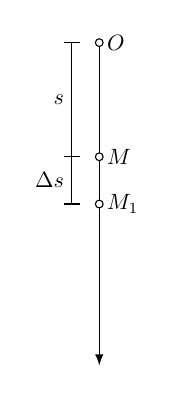
\begin{tikzpicture}[x=1cm,y=1cm]
        \draw[-latex] (0,3.1) -- (0,-1);
        \draw[fill=white] (0,3.1) circle (1.4pt) node[right,scale=0.8] {$O$};
        \draw[fill=white] (0,1.65) circle (1.4pt) node[right,scale=0.8] {$M$};
        \draw[fill=white] (0,1.05) circle (1.4pt) node[right,scale=0.8] {$M_1$};
        \draw (-0.35,3.1) -- (-0.35,1.65);
        \draw (-0.45,3.1) -- (-0.25,3.1);
        \draw (-0.45,1.65) -- (-0.25,1.65);
        \node[left,scale=0.8] at (-0.35,2.375) {$s$};
        \draw (-0.35,1.65) -- (-0.35,1.05);
        \draw (-0.45,1.05) -- (-0.25,1.05);
        \node[left,scale=0.8] at (-0.35,1.35) {$\Delta s$};
    \end{tikzpicture}
\end{wrapfigure}
给时间 $t$ 一个增量 $\Delta t>0$.
在时刻 $t+\Delta t$, 质点到达位置 $M_1$,
这段时间内的路程增量 $MM_1$ 记为 $\Delta s$.
在 \eqref{eq:free_fall_motion_law} 中用 $t+\Delta t$ 代替 $t$, 得
$$
s+\Delta s=\frac g2(t+\Delta t)^2,
$$
从而
$$
\Delta s=\frac g2(2t\Delta t+\Delta t^2).
$$
用时间增量 $\Delta t$ 除路程增量 $\Delta s$, 就得到这段时间内的\emph{平均速度}\index{pingjunsudu@平均速度}:
$$
\bar v=\frac{\Delta s}{\Delta t}=gt+\frac g2\Delta t.
$$
这个平均速度随 $\Delta t$ 而变化.
在时刻 $t$ 以后所取的时间间隔越短,
平均速度就越能反映质点在时刻 $t$ 的运动情况.

{\kaishu 当 $\Delta t$ 趋于零时, 若平均速度 $\bar v$ 有有限极限 $v$,
就称这个极限为质点在时刻 $t$ 的\emph{瞬时速度}.}
\index{shunshisudu@瞬时速度}

在当前的自由落体问题中, 有
$$
v=\lim_{\Delta t\to0}\left(gt+\frac g2\Delta t\right)=gt.
$$

类似地, 可以确定质点在一般直线运动中的速度.
质点的位置由它相对于某个固定点 $O$ 的位置量 $s$ 来确定.
时间 $t$ 从某个选定的时刻算起,
这个时刻不一定是质点位于 $O$ 的时刻.
若已知运动方程
$$
s=f(t),
$$
则质点在任意时刻的位置也就完全确定了.
在刚才的自由落体问题中, \eqref{eq:free_fall_motion_law} 就是这样的运动方程.

要确定时刻 $t$ 的速度, 仍给 $t$ 一个非零增量 $\Delta t$,
相应的位置量 $s$ 发生增量 $\Delta s$.
比值
$$
\bar v=\frac{\Delta s}{\Delta t}
$$
表示这段时间内的平均速度.
令 $\Delta t$ 趋于零, 若极限存在, 就得到时刻 $t$ 的瞬时速度:
$$
v=\lim_{\Delta t\to0}\bar v
=\lim_{\Delta t\to0}\frac{\Delta s}{\Delta t}.
$$

下面再考察另一个重要问题, 它也将引出相似的极限运算.

\subsection{切线问题}\label{subsec:91}
设有一条曲线 $(K)$ 及其上一点 $M$.
我们要建立曲线在点 $M$ 处的切线概念.

\begin{wrapfigure}[6]{l}{0.43\textwidth}
    \vspace{-0.5cm}
    \centering
    \phantomsection\label{fig:tangent_as_secant_limit}
    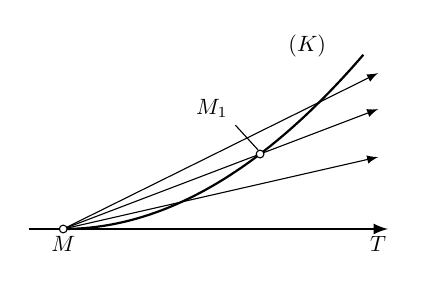
\begin{tikzpicture}[x=1.25cm,y=0.85cm]
        \draw[thick,domain=0:3.05,samples=70,smooth] plot (\x,{0.28*\x*\x});
        \draw[-latex] (0,0) -- (3.2,1.0752);
        \draw[-latex] (0,0) -- (3.2,1.792);
        \draw[-latex] (0,0) -- (3.2,2.3296);
        \draw[thick,-latex] (-0.35,0) -- (3.3,0);
        \draw[fill=white] (0,0) circle (1.4pt) node[below,scale=0.8] {$M$};
        \draw[fill=white] (2,1.12) circle (1.4pt);
        \draw (1.75,1.55) -- (1.98,1.18);
        \node[above left,scale=0.8] at (1.75,1.55) {$M_1$};
        \node[above left,scale=0.8] at (2.75,2.45) {$(K)$};
        \node[below,scale=0.8] at (3.2,0) {$T$};
    \end{tikzpicture}
\end{wrapfigure}
中学里常把圆的切线说成“与圆只有一个公共点的直线”.
但这个说法具有特殊性, 不能说明一般曲线相切的本质.
例如, 对抛物线 $y=ax^2$ ($a>0$), 两个坐标轴都只在原点 $O$ 与它相交,
因而都符合上述说法; 但实际在原点与抛物线相切的只有 $x$ 轴.

现在给出一般的定义.
在曲线 $(K)$ 上另取一点 $M_1\ne M$, 作\emph{割线}\index{gexian@割线} $MM_1$.
当 $M_1$ 沿曲线向 $M$ 移动时, 这条割线就绕着 $M$ 转动, 如图所示.

\phantomsection\label{def:tangent_line}
{\kaishu 当点 $M_1$ 沿曲线 $(K)$ 趋于点 $M$ 时,
若割线 $MM_1$ 有极限位置 $MT$,
就称直线 $MT$ 为曲线 $(K)$ 在点 $M$ 处的\emph{切线}.}
\index{qiexian@切线}
这里所谓极限位置, 是说只要弦 $MM_1$ 足够短,
割线 $MM_1$ 与直线 $MT$ 所成的角就可以任意小.

例如, 求抛物线
$$
y=ax^2
$$
在任意点 $M(x,y)$ 处的切线.
因为切线经过 $M$, 所以只须再确定它的\emph{斜率}\index{xielv@斜率}, 就能确定这条直线的位置.
下图中取 $a>0$.

\begin{figure}[!ht]
    \centering
    \phantomsection\label{fig:parabola_tangent_construction}
    \begin{minipage}{0.48\textwidth}
        \centering
        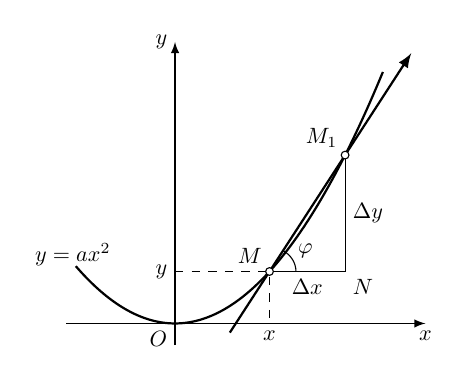
\begin{tikzpicture}[x=1.2cm,y=1.1cm]
            \draw[-latex] (-1.15,0) -- (2.65,0) node[below,scale=0.8] {$x$};
            \draw[-latex] (0,-0.25) -- (0,3.25) node[left,scale=0.8] {$y$};
            \draw[thick,domain=-1.05:2.2,samples=80,smooth] plot (\x,{0.6*\x*\x});
            \draw[thick,-latex] (0.58,-0.1056) -- (2.5,3.12);
            \draw[dashed] (0,0.6) -- (1,0.6) -- (1,0);
            \draw (1,0.6) -- (1.8,0.6) -- (1.8,1.944);
            \draw[fill=white] (1,0.6) circle (1.4pt) node[above left,scale=0.8] {$M$};
            \draw[fill=white] (1.8,1.944) circle (1.4pt) node[above left,scale=0.8] {$M_1$};
            \node[below right,scale=0.8] at (1.8,0.6) {$N$};
            \node[below left,scale=0.8] at (0,0) {$O$};
            \node[below,scale=0.8] at (1,0) {$x$};
            \node[left,scale=0.8] at (0,0.6) {$y$};
            \node[below,scale=0.8] at (1.4,0.6) {$\Delta x$};
            \node[right,scale=0.8] at (1.8,1.27) {$\Delta y$};
            \node[left,scale=0.8] at (-0.6,0.8) {$y=ax^2$};
            \draw (1.28,0.6) arc (0:59.237:0.28);
            \node[above right,scale=0.8] at (1.22,0.67) {$\varphi$};
        \end{tikzpicture}
        \par\smallskip $(a)$
    \end{minipage}\hfill
    \begin{minipage}{0.48\textwidth}
        \centering
        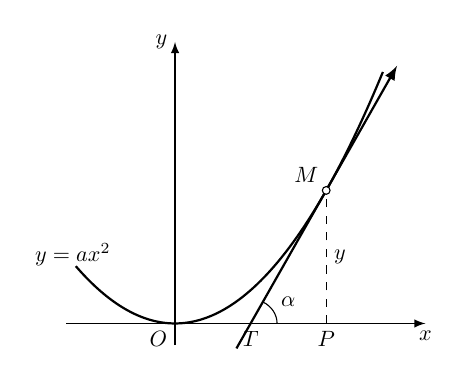
\begin{tikzpicture}[x=1.2cm,y=1.1cm]
            \draw[-latex] (-1.15,0) -- (2.65,0) node[below,scale=0.8] {$x$};
            \draw[-latex] (0,-0.25) -- (0,3.25) node[left,scale=0.8] {$y$};
            \draw[thick,domain=-1.05:2.2,samples=80,smooth] plot (\x,{0.6*\x*\x});
            \draw[thick,-latex] (0.65,-0.288) -- (2.35,2.976);
            \draw[dashed] (1.6,0) -- (1.6,1.536);
            \draw[fill=white] (1.6,1.536) circle (1.4pt) node[above left,scale=0.8] {$M$};
            \node[below left,scale=0.8] at (0,0) {$O$};
            \node[below,scale=0.8] at (0.8,0) {$T$};
            \node[below,scale=0.8] at (1.6,0) {$P$};
            \node[right,scale=0.8] at (1.6,0.77) {$y$};
            \node[left,scale=0.8] at (-0.6,0.8) {$y=ax^2$};
            \draw (1.08,0) arc (0:62.488:0.28);
            \node[above right,scale=0.8] at (1.04,0.1) {$\alpha$};
        \end{tikzpicture}
        \par\smallskip $(b)$
    \end{minipage}
\end{figure}

给横坐标 $x$ 一个非零增量 $\Delta x$, 就从点 $M$ 移到曲线上的另一点 $M_1$.
它的横坐标为 $x+\Delta x$, 纵坐标为
$$
y+\Delta y=a(x+\Delta x)^2.
$$
在图 $(a)$ 的直角三角形 $MNM_1$ 中,
水平边 $MN$ 对应横坐标增量 $\Delta x$, 竖直边 $NM_1$ 对应纵坐标增量 $\Delta y$.
由抛物线方程得到
$$
\Delta y=a(2x\Delta x+\Delta x^2),
$$
所以割线 $MM_1$ 的斜率为
$$
\tan\varphi=\frac{\Delta y}{\Delta x}=2ax+a\Delta x.
$$
要求切线的斜率, 就令 $\Delta x\to0$, 得
$$
\tan\alpha=\lim_{\Delta x\to0}(2ax+a\Delta x)=2ax.
$$

顺便指出, 由此还能得到实际作这条切线的简便方法.
在图 $(b)$ 中, $P$ 是 $M$ 在 $x$ 轴上的投影, $T$ 是切线与 $x$ 轴的交点.
对于图中 $x>0$ 的情形, 由直角三角形 $MPT$ 有
$$
TP=\frac{y}{\tan\alpha}=\frac{ax^2}{2ax}=\frac x2.
$$
因此 $T$ 是线段 $OP$ 的中点.
于是, 把线段 $OP$ 二等分, 再把中点 $T$ 与 $M$ 连接起来, 就得到所求的切线.
在原点 $O$ 处, 切线就是 $x$ 轴.

对于一般曲线, 若已知方程
$$
y=f(x),
$$
也可以用相同的方法求切线的斜率.
与横坐标增量 $\Delta x$ 对应的纵坐标增量记为 $\Delta y$,
则比值 $\Delta y/\Delta x$ 就是割线的斜率 $\tan\varphi$.
当 $\Delta x\to0$ 时, 若这个比值有有限极限, 就得到切线的斜率:
$$
\tan\alpha=\lim_{\Delta x\to0}\tan\varphi
=\lim_{\Delta x\to0}\frac{\Delta y}{\Delta x}.
$$
